\documentclass[aspectratio=169,t,11pt,table]{beamer}
\usepackage{../../slides}
\usepackage{../../math}
\usepackage{../../uark_colors}

\definecolor{accent}{HTML}{9D2235}
\definecolor{accent2}{HTML}{2B5269}

\title{Topic 1: Introduction to Forecasting}
\subtitle{\it  ECON 4753 — University of Arkansas}
\date{Fall 2024}
\author{Prof. Kyle Butts}

\begin{document}

% ------------------------------------------------------------------------------
\begin{frame}[noframenumbering,plain]
\maketitle

% \bottomleft{\footnotesize $^*$A bit of extra info here. Add an asterich to title or author}
\end{frame}
% ------------------------------------------------------------------------------

\begin{frame}{}
  \bigskip\bigskip
  \begin{center}
    \alert{\LARGE\bf Welcome to Forecasting (Econ 4753)}
  \end{center}

  \bigskip\bigskip
  Who am I?
  \begin{itemize}
    \item Kyle Butts, Ph.D.; please call me Kyle
    
    \item Graduated from University of Colorado Boulder
    
    \item Research: 
    \begin{itemize}
      \item Econometrics and Causal Inference
      \item Housing economics (e.g. zoning laws and landords)
    \end{itemize}
  \end{itemize}
\end{frame}

\begin{frame}{Classroom Norms}
  \begin{enumerate}
    \item All \alert{\bf questions are appreciated}. 
    \begin{itemize}
      \item I \emph{always} have time to answer them.
    \end{itemize}

    \item If you can not \alert{\bf stay off the internet during class}, do not come to class. 
    \begin{itemize}
      \item I do not take attendance and it is not fair to other students.
    \end{itemize}
    
    \item This class has \alert{\bf coding exercises} in R. 
    \begin{itemize}
      \item Bring your laptop so you can participate
      
      \item We will introduce R, but you will need to put in some time outside of class to practice. 
      
      \item Coding is becoming increasingly valuable for your career; it is a competitive advantage on the job market.
    \end{itemize}
  \end{enumerate}
\end{frame}

\begin{frame}{Course Materials}{Coding Software}
  You will need to download \emph{two} programs:
  \begin{enumerate}
    \item Install R from \url{https://cloud.r-project.org/}.
    \item Install Positron (or RStudio) from \url{https://github.com/posit-dev/positron/releases}. 
  \end{enumerate}

  \bigskip
  Your first assignment will be to download the software and compile an \texttt{.Rmd} file.
\end{frame}

\begin{frame}{Course Materials}{Textbooks}
  Both textbooks are available for free online:
  \begin{enumerate}
    \item Gareth, J., Daniela, W., Trevor, H., \& Robert, T. (2013). ``An introduction to statistical learning: with applications in R (2nd edition)''. Spinger.
    
    \item Hyndman, R. J., \& Athanasopoulos, G. (2018). ``Forecasting: principles and practice (3rd edition)''. OTexts.
  \end{enumerate}

  \bigskip
  We will also have some readings from Nate Silver's book which I'll post snippets for you:
  \begin{itemize}
    \item Silver, N. (2012). ``The signal and the noise: Why so many predictions fail-but some don't''. Penguin.
  \end{itemize}
\end{frame}

\begin{frame}{Assignments}
  \begin{enumerate}
    \item There will be a set of assignments in this course roughly following each Topic.
    \begin{itemize}
      \item Assignments will have a mixture of free-response questions and coding exercises
    \end{itemize}

    \item Two midterms and one final:
    \begin{itemize}
      \item Midterms are non-cumulative; final is cumulative
    \end{itemize}
  \end{enumerate}
\end{frame}

\begin{frame}{Grading}
  TBD
\end{frame}





% ------------------------------------------------------------------------------
\section{Motivation}
% ------------------------------------------------------------------------------

\begin{frame}{Key elements of forecasting}
  Forecasting is the use of data to make predictions about an uncertain/unobserved outcome

  \bigskip
  Typically, it is a mix of two \emph{important components}
  \begin{enumerate}
    \item An estimate, usually a number or a set of numbers that summarize the prediction
    
    \item A measure of uncertainty, reflecting how variable we think our estimate is
    \begin{itemize}
      \item Want to communicate to stakeholders how confident in our estimate we are
    \end{itemize}
  \end{enumerate}

  Let's look at some examples and try to identify forecasts and their measures of uncertainty (if any)
\end{frame}

\begin{frame}{Election Forecasting}
  \begin{columns}[T]
    \begin{column}{.7\textwidth}\vspace*{-\bigskipamount}
      \begin{center}
        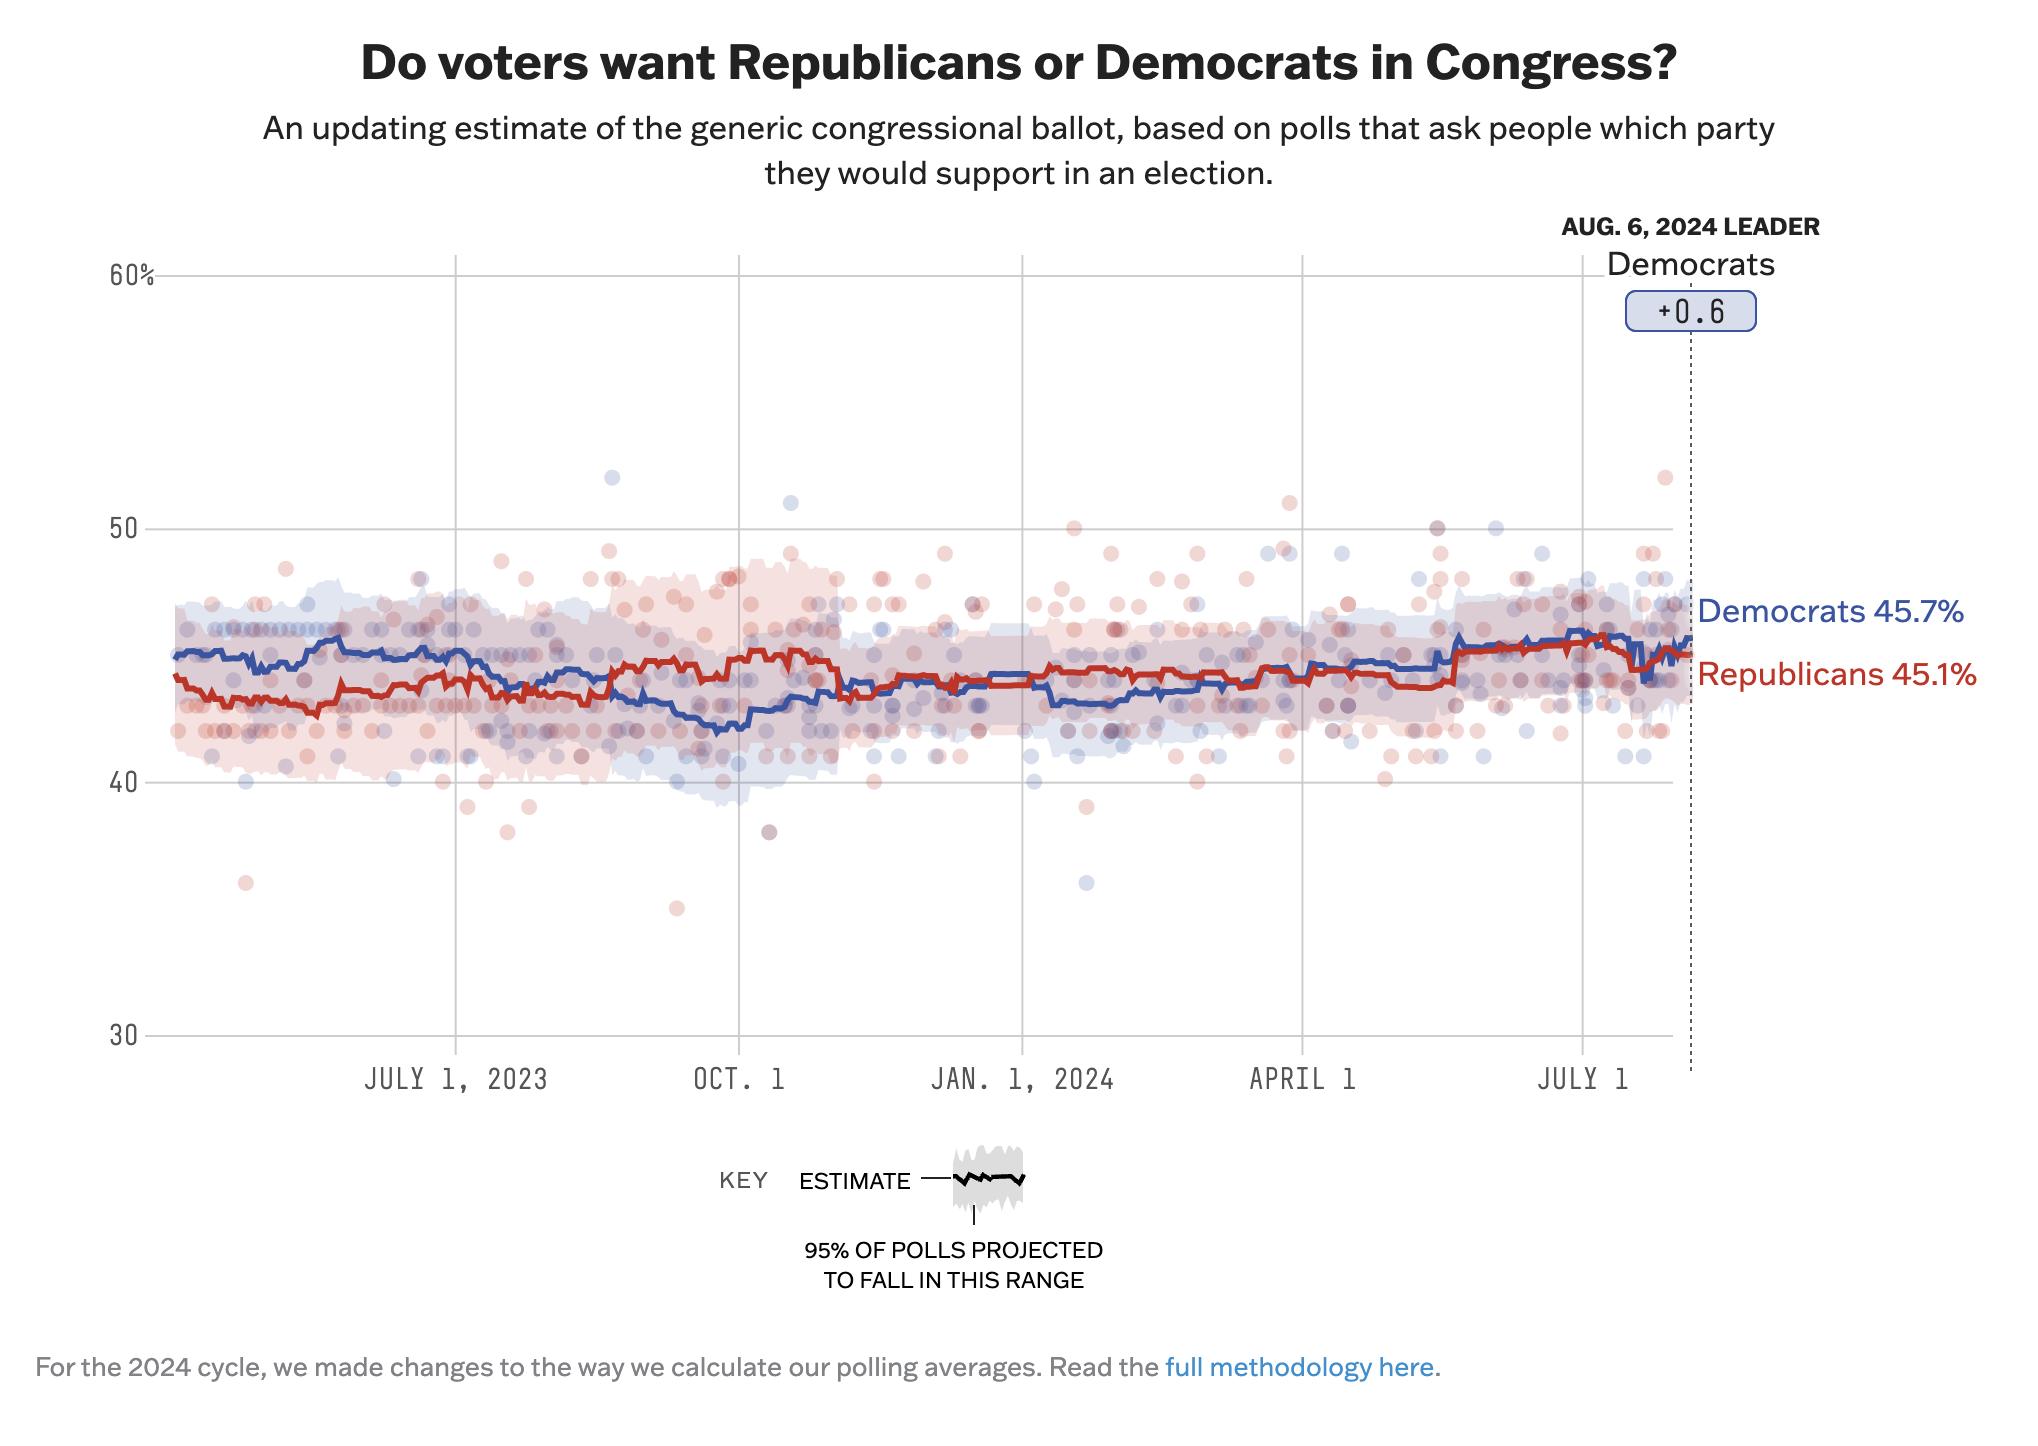
\includegraphics[width = 0.85\textwidth]{figures/polling_timeseries.png}
      \end{center}
    \end{column}
    \begin{column}{.3\textwidth}
      Source:

      \href{https://www.natesilver.net/p/nate-silver-2024-president-election-polls-model}{Nate Silver's Blog}
    \end{column}
  \end{columns}
\end{frame}

\begin{frame}{Election Forecasting}
  \begin{columns}[T]
    \begin{column}{.7\textwidth}\vspace*{-\bigskipamount}
      \begin{center}
        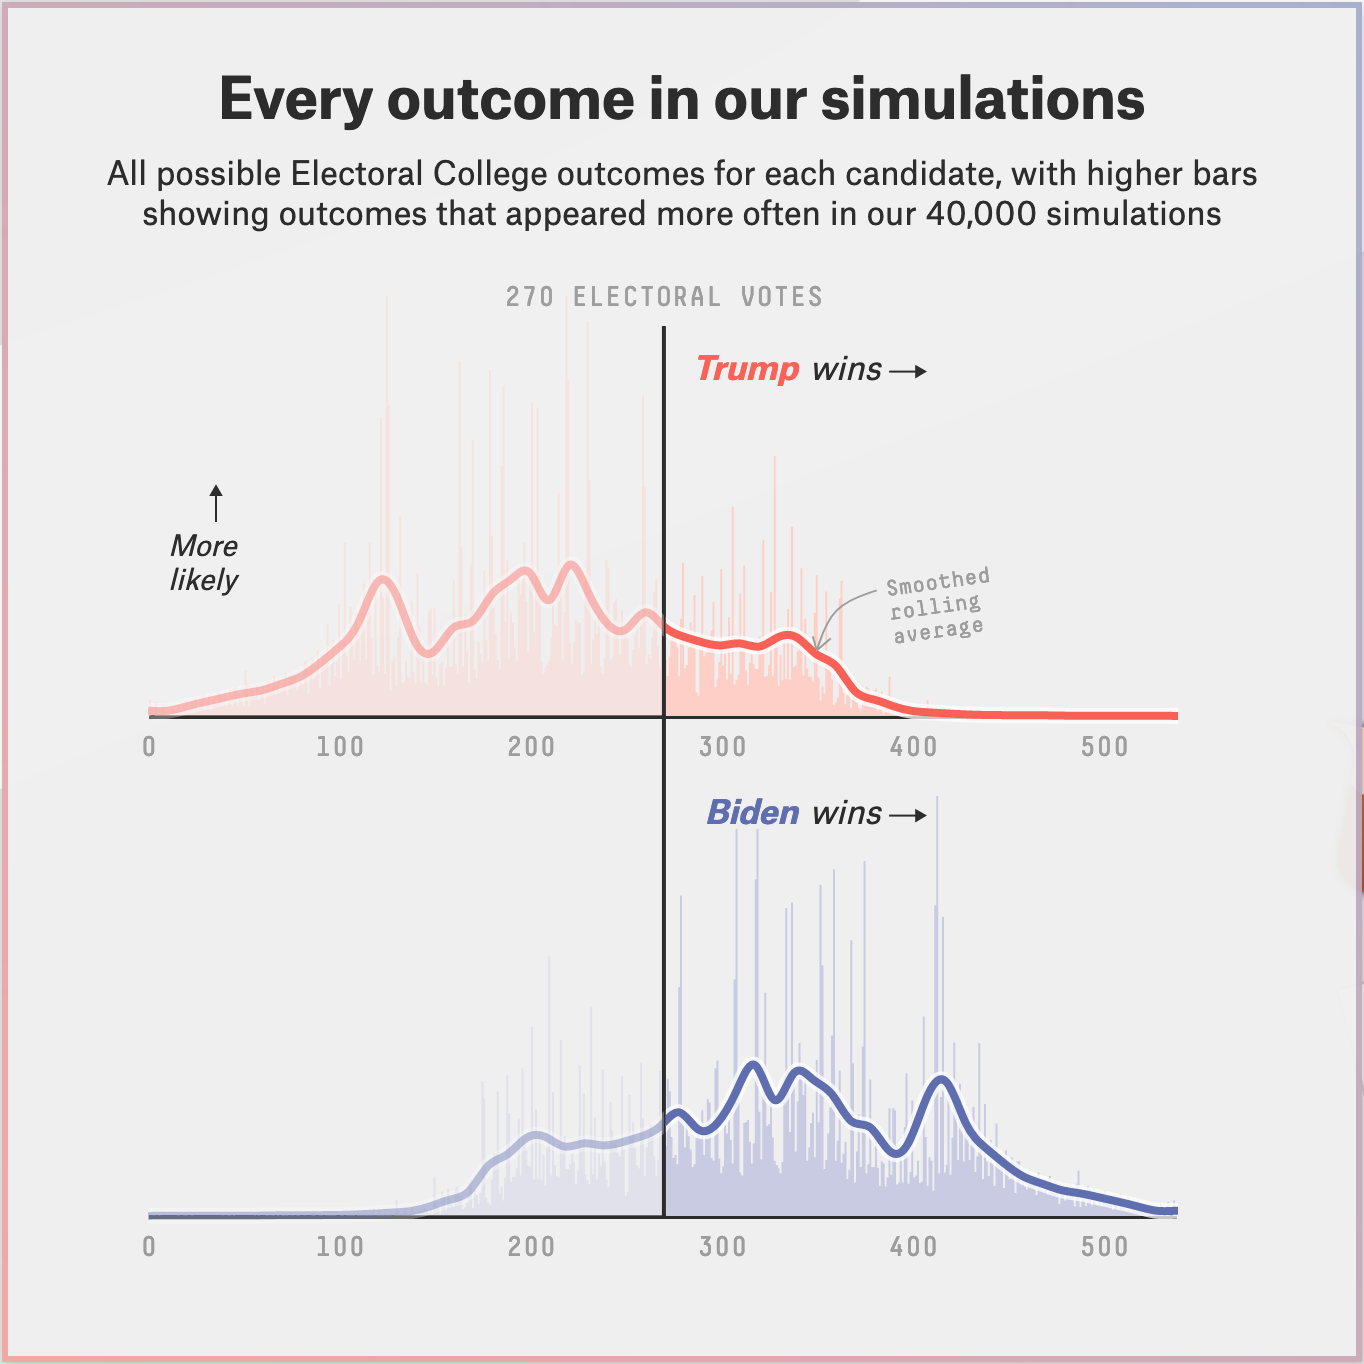
\includegraphics[width = 0.65\textwidth]{figures/538_3.png}
      \end{center}
    \end{column}
    \begin{column}{.3\textwidth}
      Source:

      \href{https://projects.fivethirtyeight.com/2020-election-forecast/}{538 2020 Election forecase}
    \end{column}
  \end{columns}
\end{frame}

\begin{frame}{Weather Predictions}
  \begin{columns}[T]
    \begin{column}{.7\textwidth}\vspace*{-\bigskipamount}
      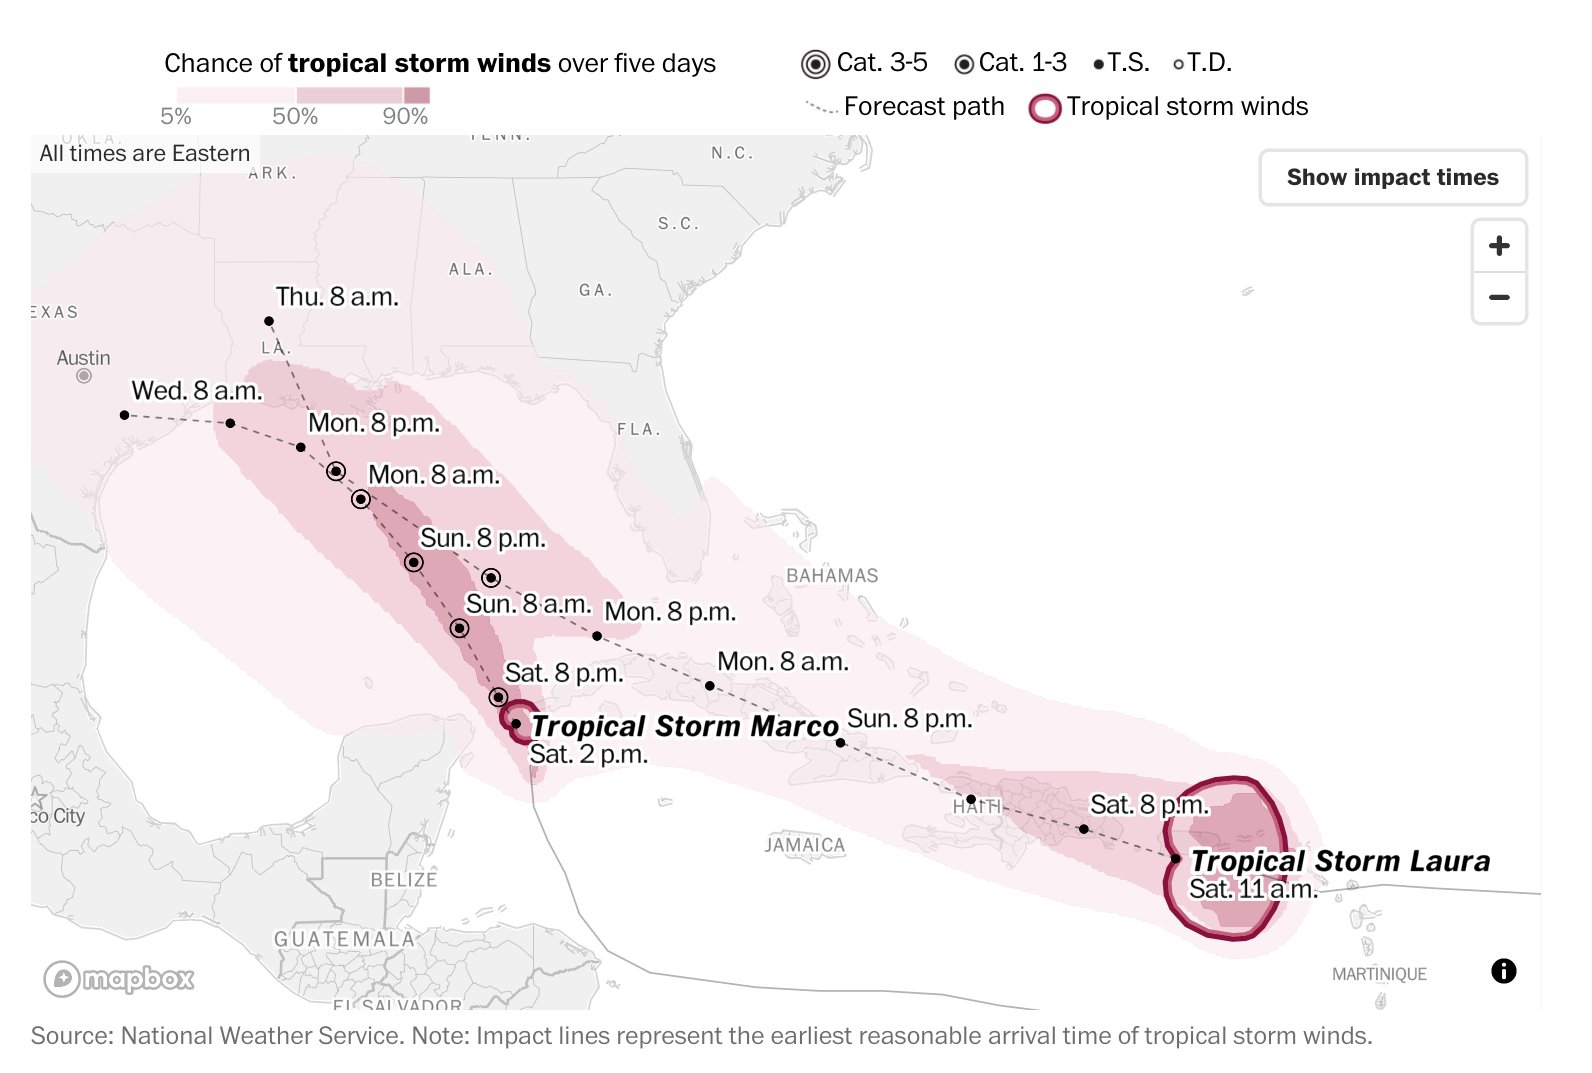
\includegraphics[width = \textwidth]{figures/hurricane.jpg}
    \end{column}
    \begin{column}{.3\textwidth}
      Source:

      \href{https://www.washingtonpost.com/weather/2020/08/21/gulf-coast-hurricanes/}{Washington Post}
    \end{column}
  \end{columns}
\end{frame}

\begin{frame}{Weather Predictions}
  \begin{columns}[T]
    \begin{column}{.7\textwidth}\vspace*{-\bigskipamount}
      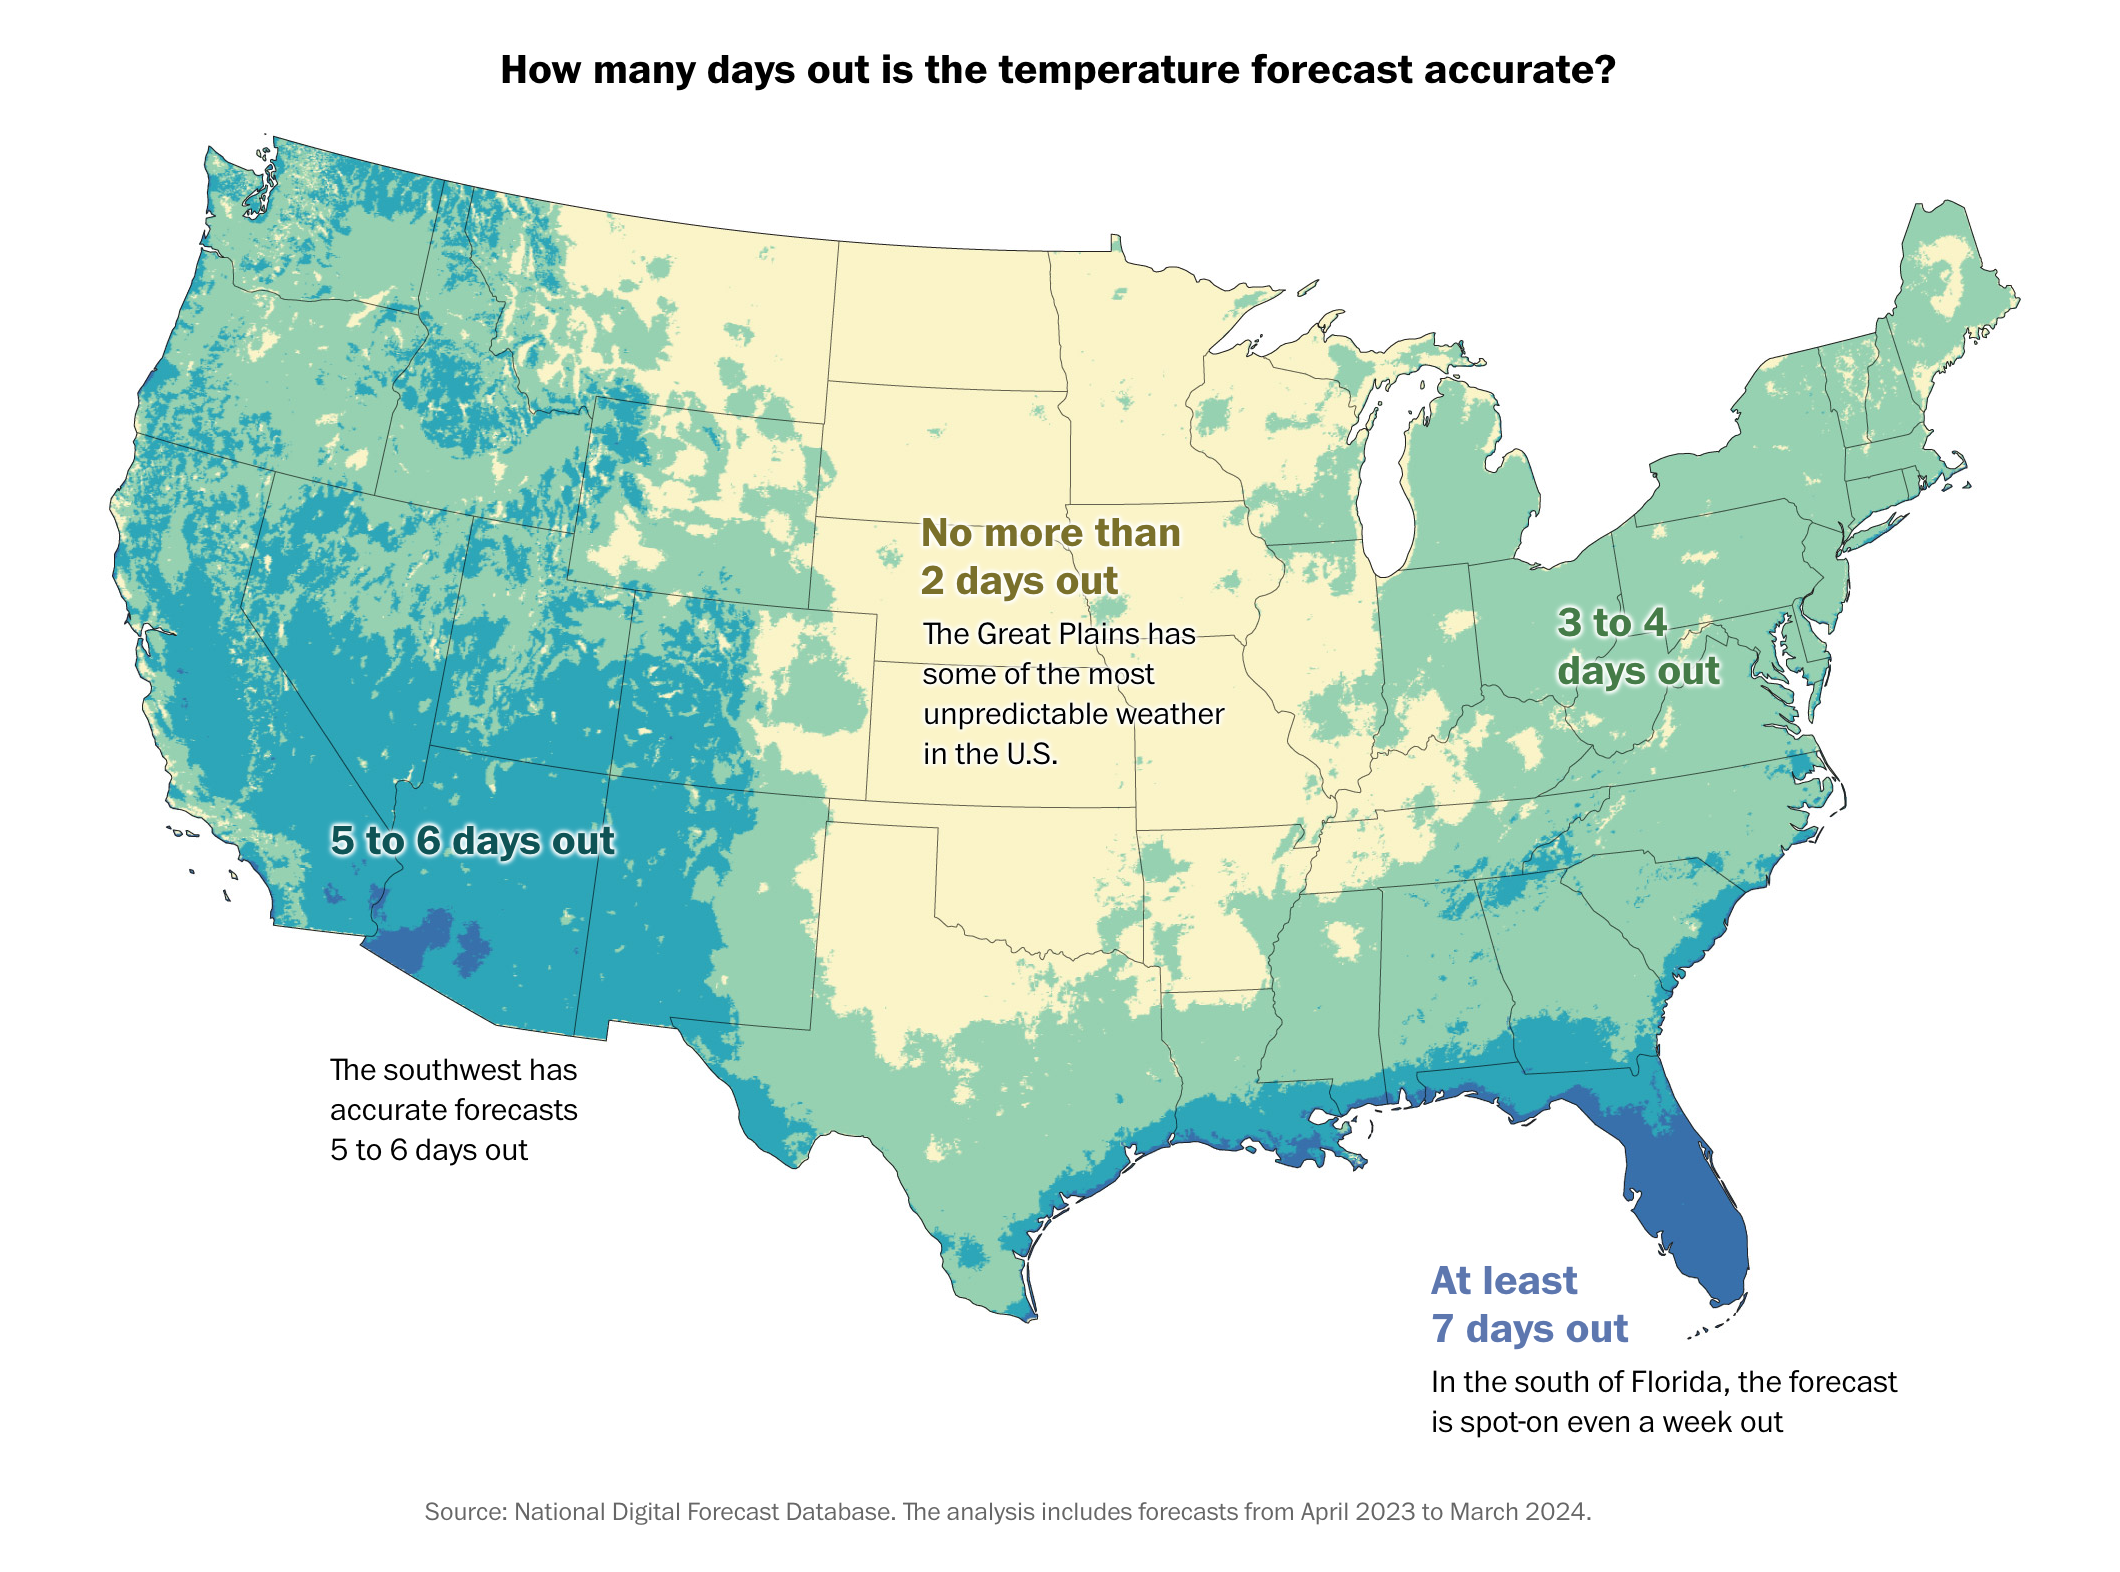
\includegraphics[width = 0.9\textwidth]{figures/how_reliable_weather_forecasts.png}
    \end{column}
    \begin{column}{.3\textwidth}
      Source:

      \href{https://www.washingtonpost.com/climate-environment/interactive/2024/how-accurate-is-the-weather-forecast/}{Washington Post}
    \end{column}
  \end{columns}
\end{frame}

\begin{frame}{Business Analytics}
  \begin{columns}[T]
    \begin{column}{.7\textwidth}\vspace*{-\bigskipamount}
      \begin{center}
        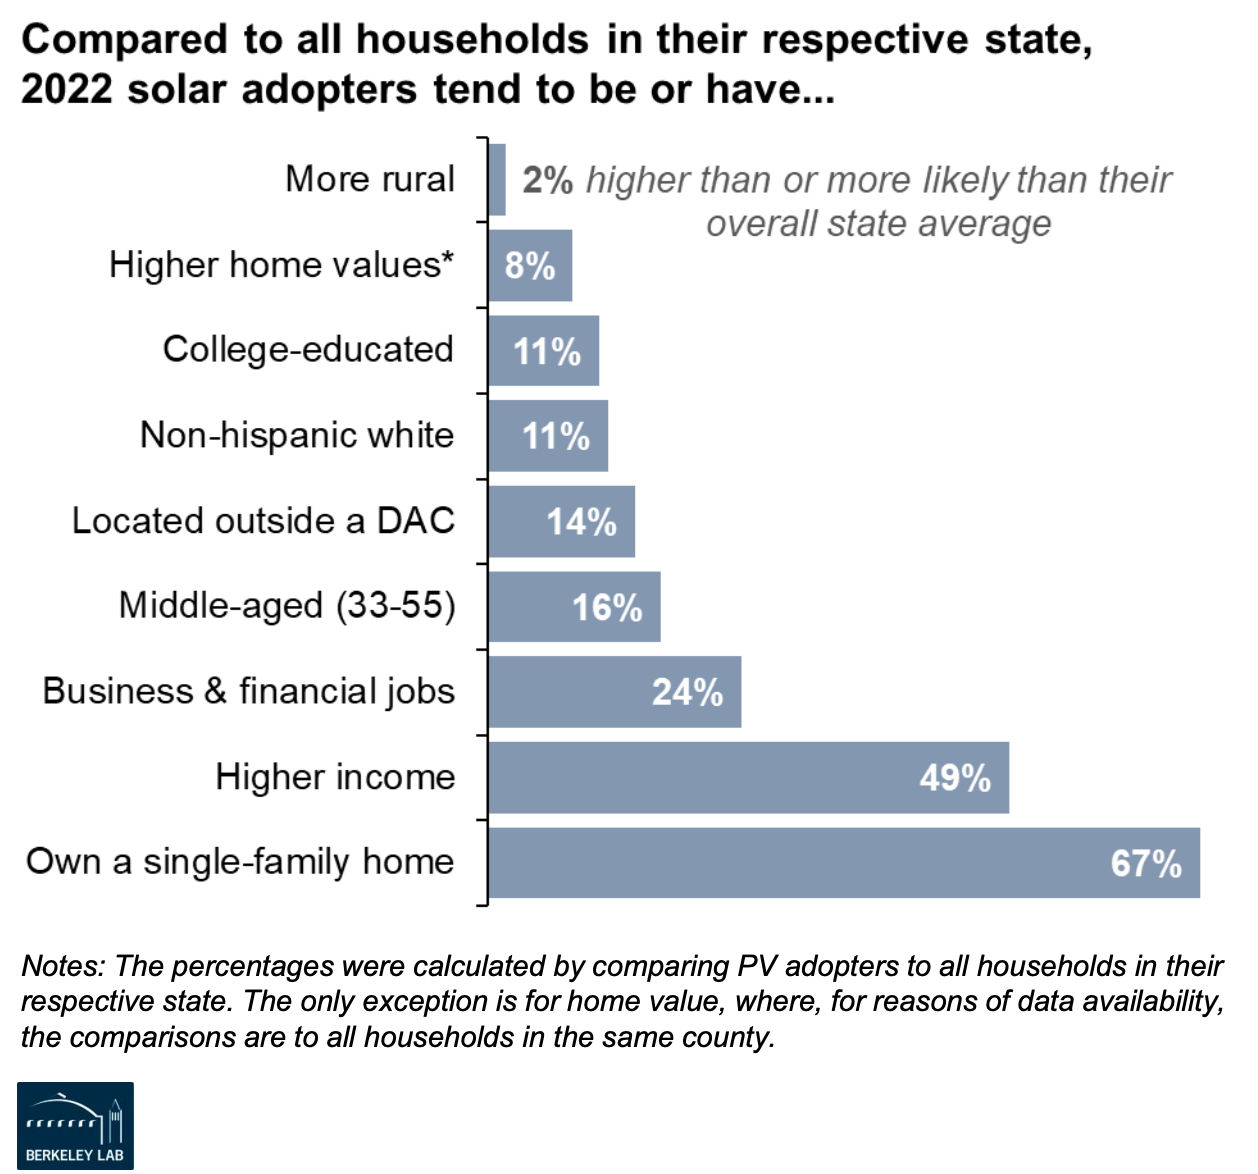
\includegraphics[width = 0.7\textwidth]{figures/solar_demand.png}
      \end{center}
    \end{column}
    \begin{column}{.3\textwidth}
      Source:

      \href{https://emp.lbl.gov/solar-demographics-tool}{Lawrence Berkeley Lab}
    \end{column}
  \end{columns}
\end{frame}

\begin{frame}{Business Analytics}
  \begin{columns}[T]
    \begin{column}{.7\textwidth}\vspace*{-1.5\bigskipamount}
      \begin{center}
        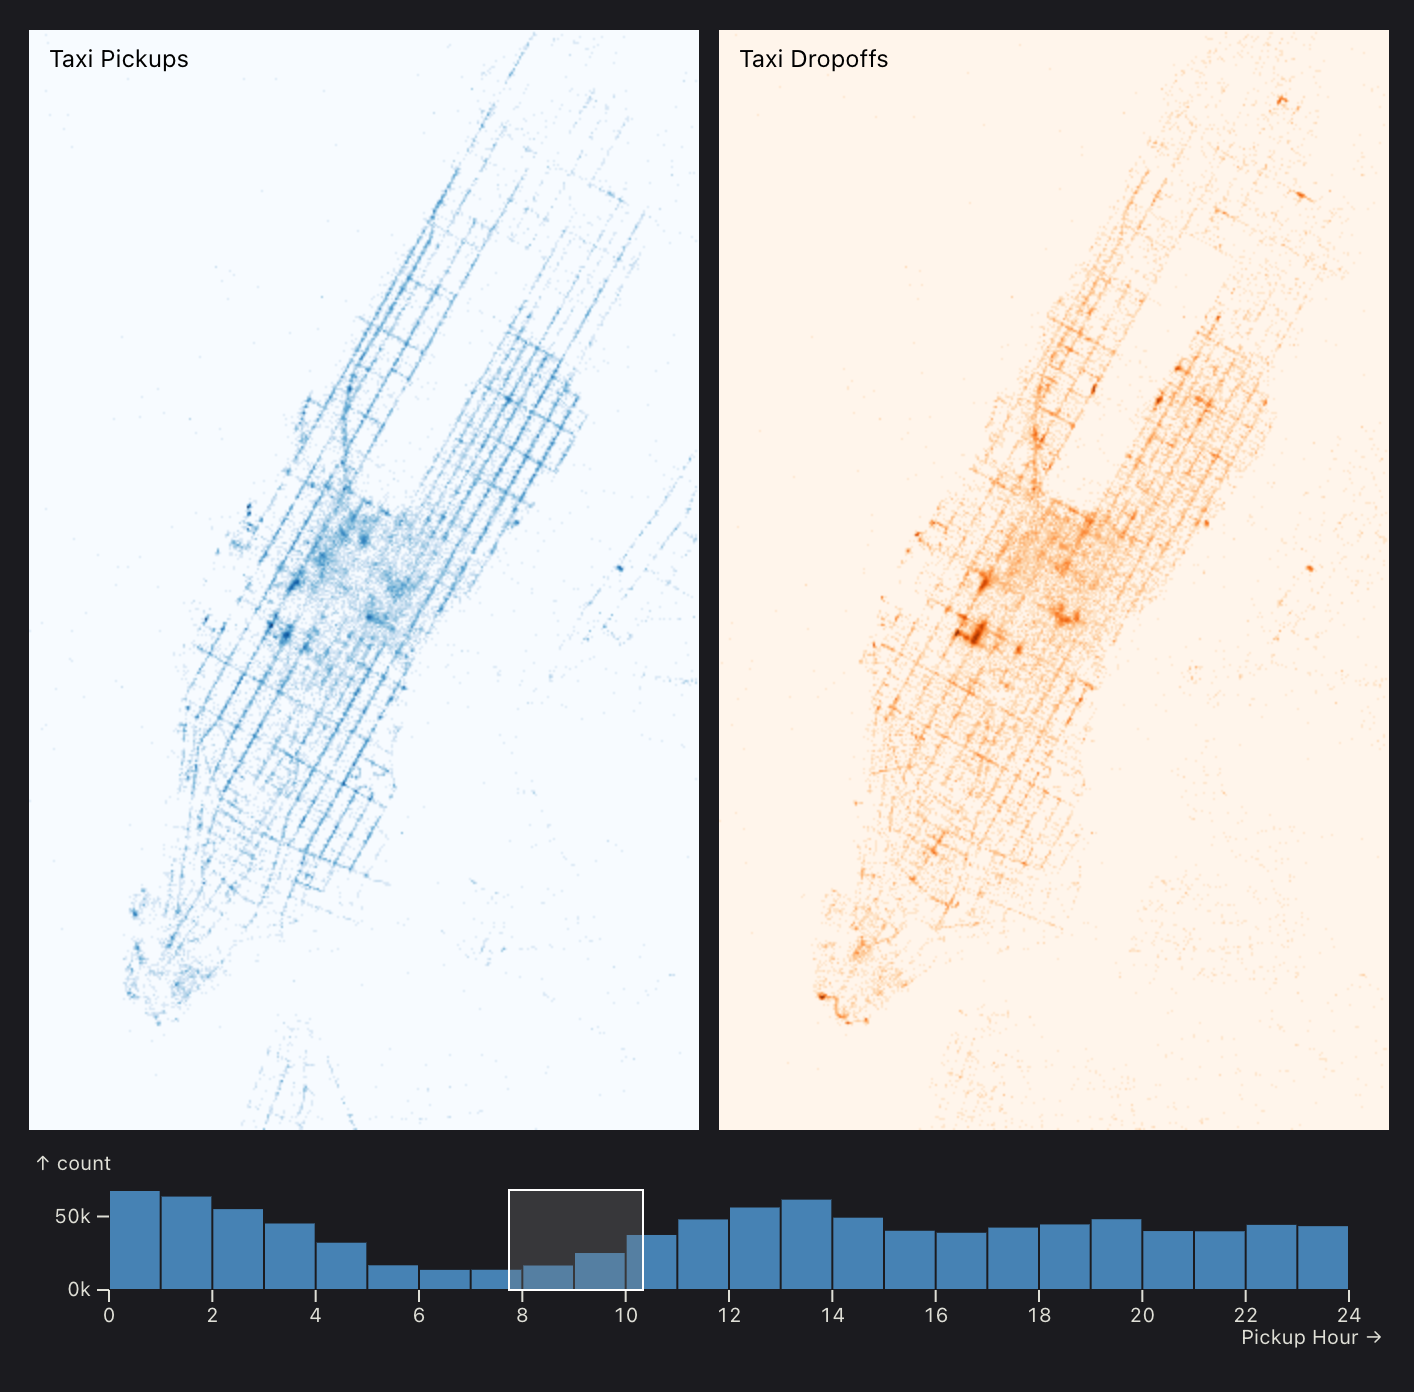
\includegraphics[width = 0.67\textwidth]{figures/nyc_taxis.png}
      \end{center}
    \end{column}
    \begin{column}{.3\textwidth}
      Source:

      \href{https://idl.uw.edu/mosaic/examples/nyc-taxi-rides.html}{Mosaic Dashboard}
    \end{column}
  \end{columns}
\end{frame}

\begin{frame}{Sports Analytics}
  \begin{columns}[T]
    \begin{column}{.7\textwidth}\vspace*{-1.5\bigskipamount}
      \begin{center}
        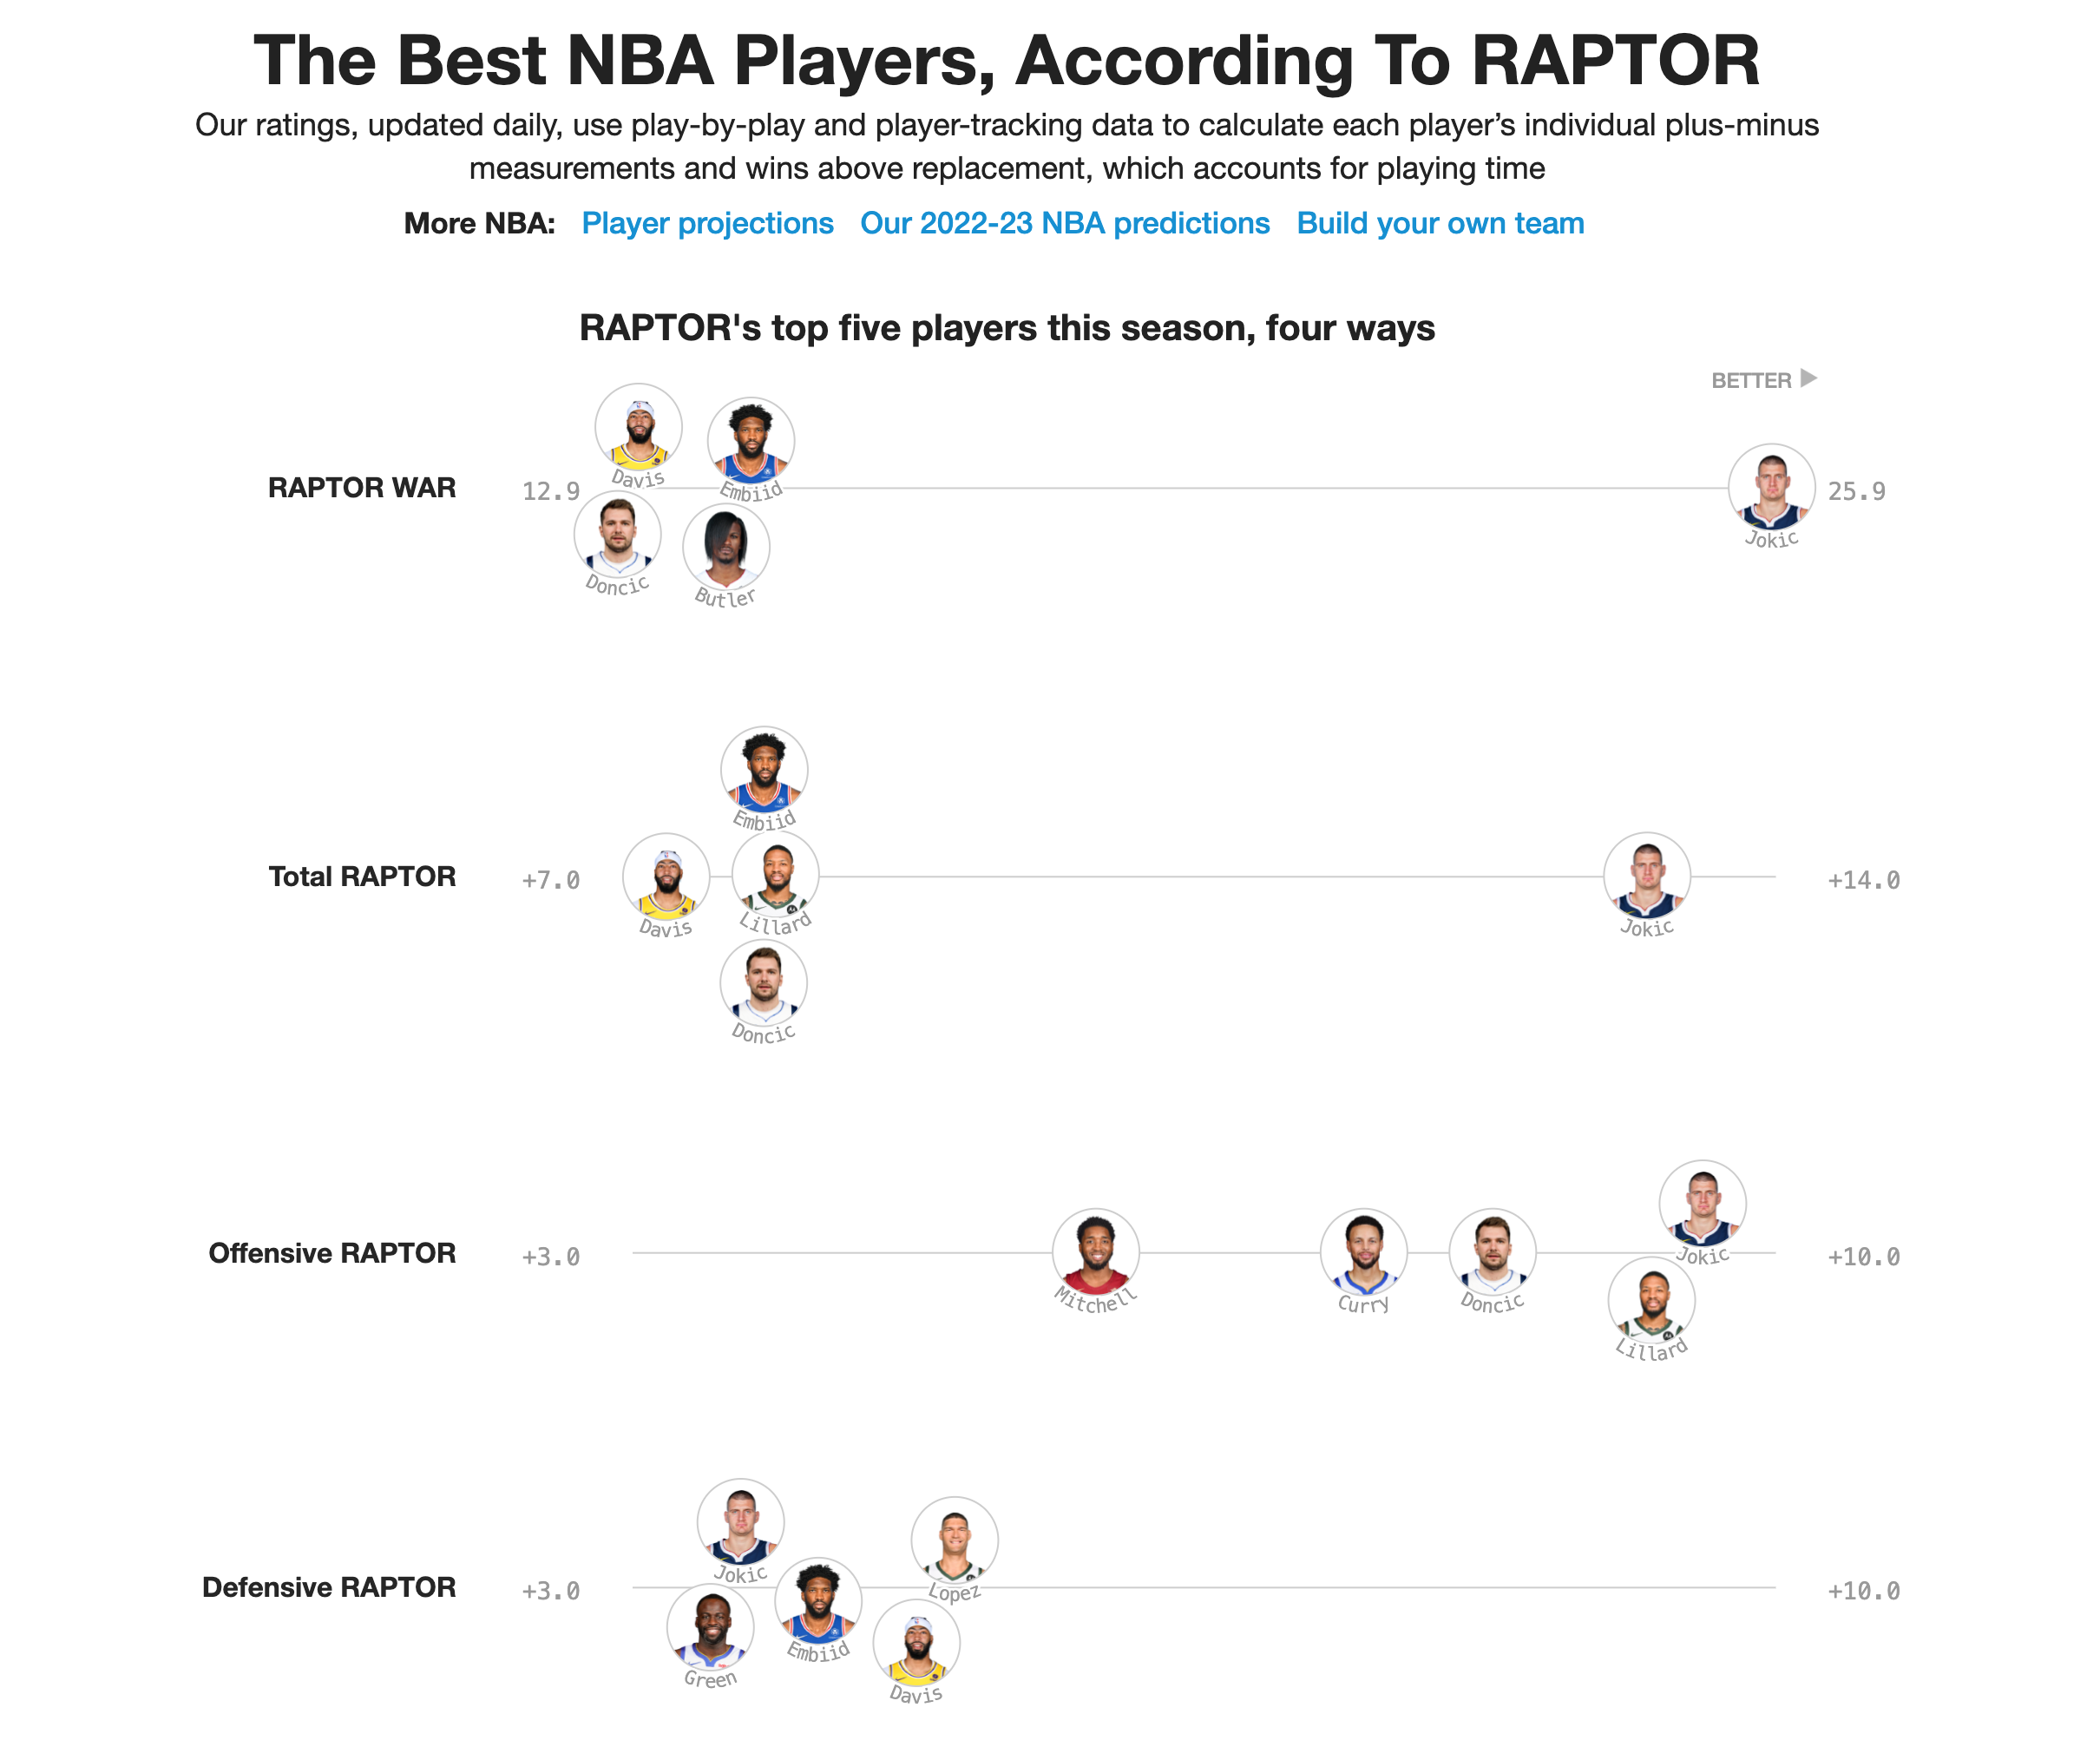
\includegraphics[width = 0.8\textwidth]{figures/nba_raptor.png}
      \end{center}
    \end{column}
    \begin{column}{.3\textwidth}
      Source:

      \href{https://projects.fivethirtyeight.com/nba-player-ratings/}{538 Player Ratings Dashboard}
    \end{column}
  \end{columns}
\end{frame}



\section*{Conclusion}

\begin{frame}{Next Topic}
  The next topic will review:
  \begin{itemize}
    \item Algebra skills that will be required in the course
    
    \item Review material from your introductory statistics class
  \end{itemize}

  \bigskip
  We will cover the material realtively quickly; ultimately, it is your job to make sure you are up to date with this material
  \begin{itemize}
    \item Come to office hours if you want to review with me in more detail
  \end{itemize}
\end{frame}


\end{document}
